%%%%%%%%%%%%%%%%%
% Getting Started
%%%%%%%%%%%%%%%%%

\section{Getting Started}
\label{sec:getting_started}

%%%%%%%%%%
% Examples
%%%%%%%%%%
\section{Examples}
\label{sec:examples}

\subsection{\LaTeX\ Examples}
\label{sec:latex_examples}

\subsection{Math Examples}
\label{sec:math_examples}

\subsection{TikZ Examples}
\label{sec:tikz_examples}

\subsubsection{Including Images}
\label{sec:including_images}
Here is an example of how to include an image:
\begin{lstlisting}
\begin{center}
    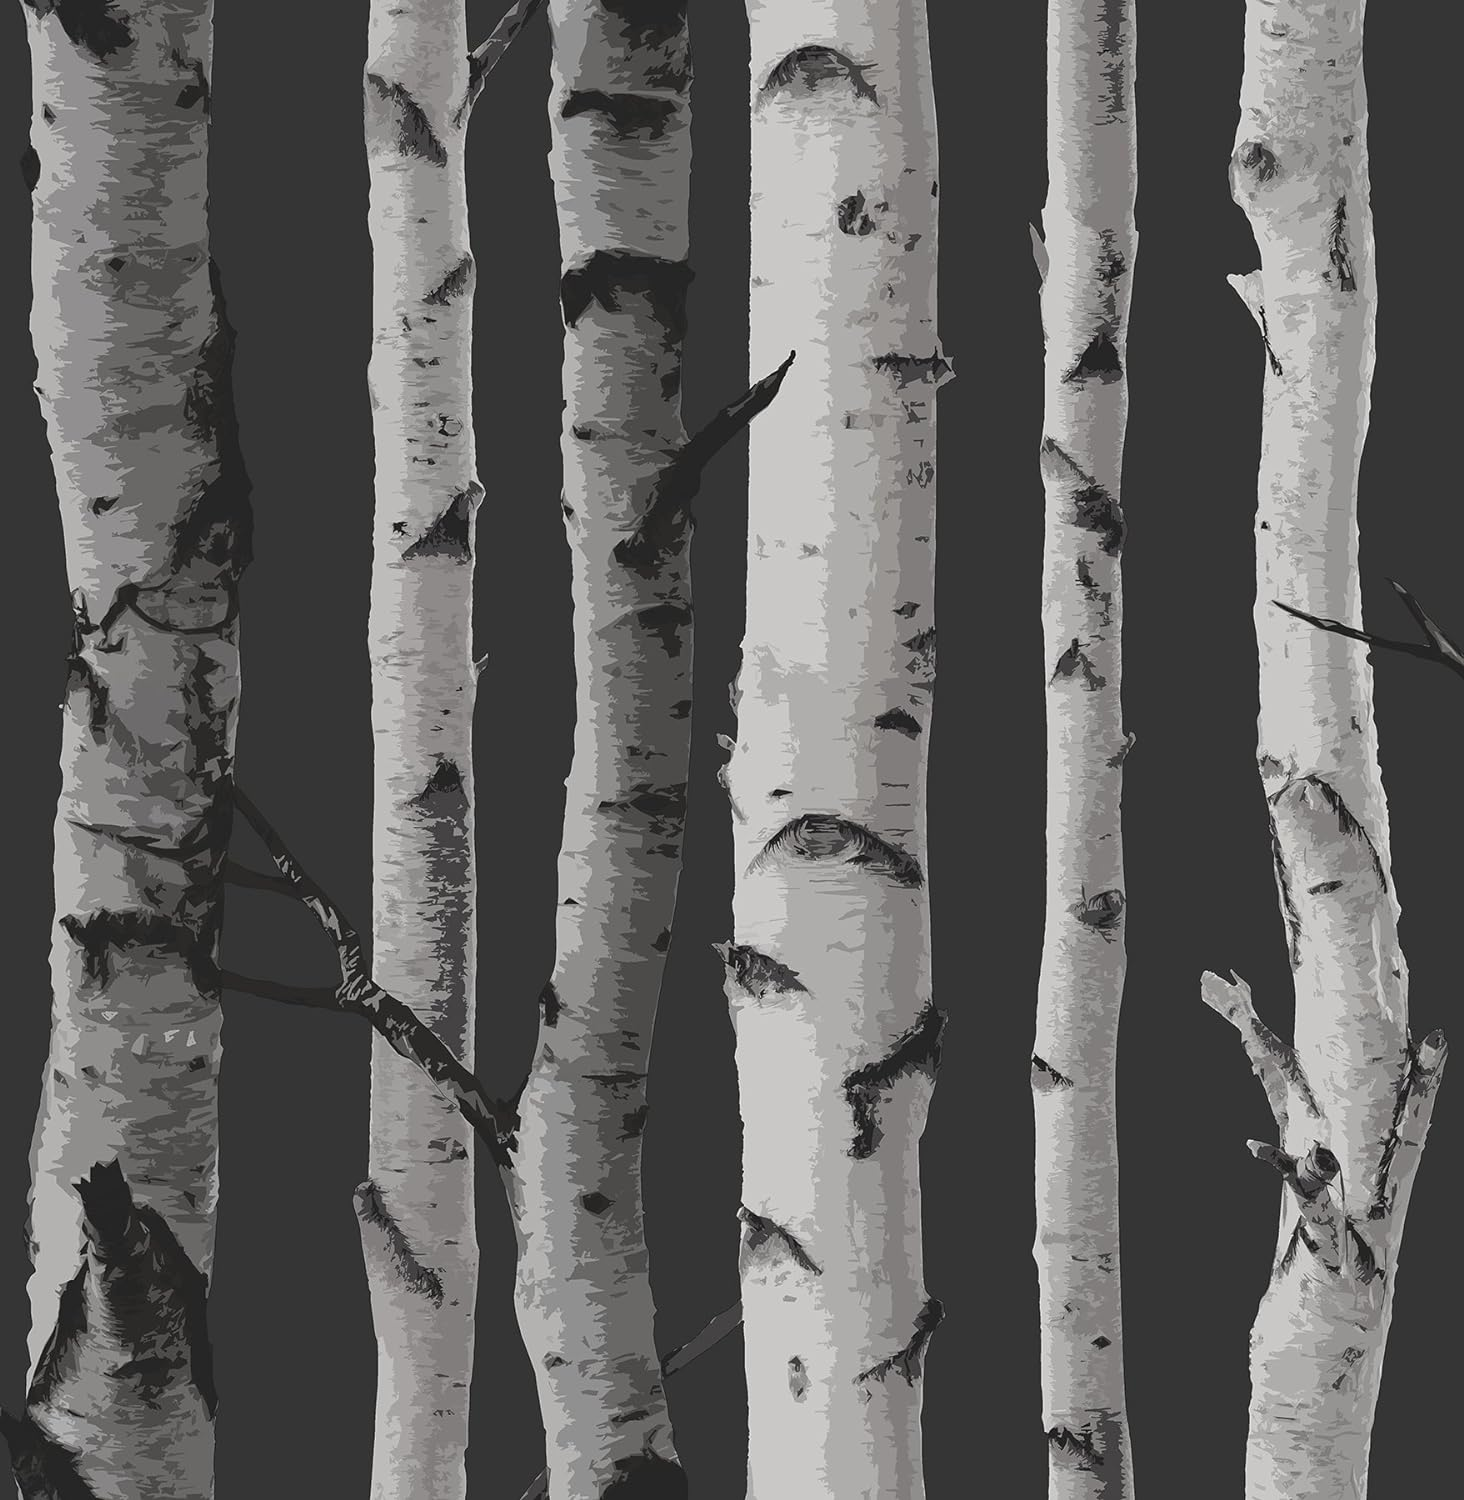
\includegraphics[width=0.5\linewidth]{birch.jpg}
\end{center}
\end{lstlisting}
This code renders the following:
\begin{center}
    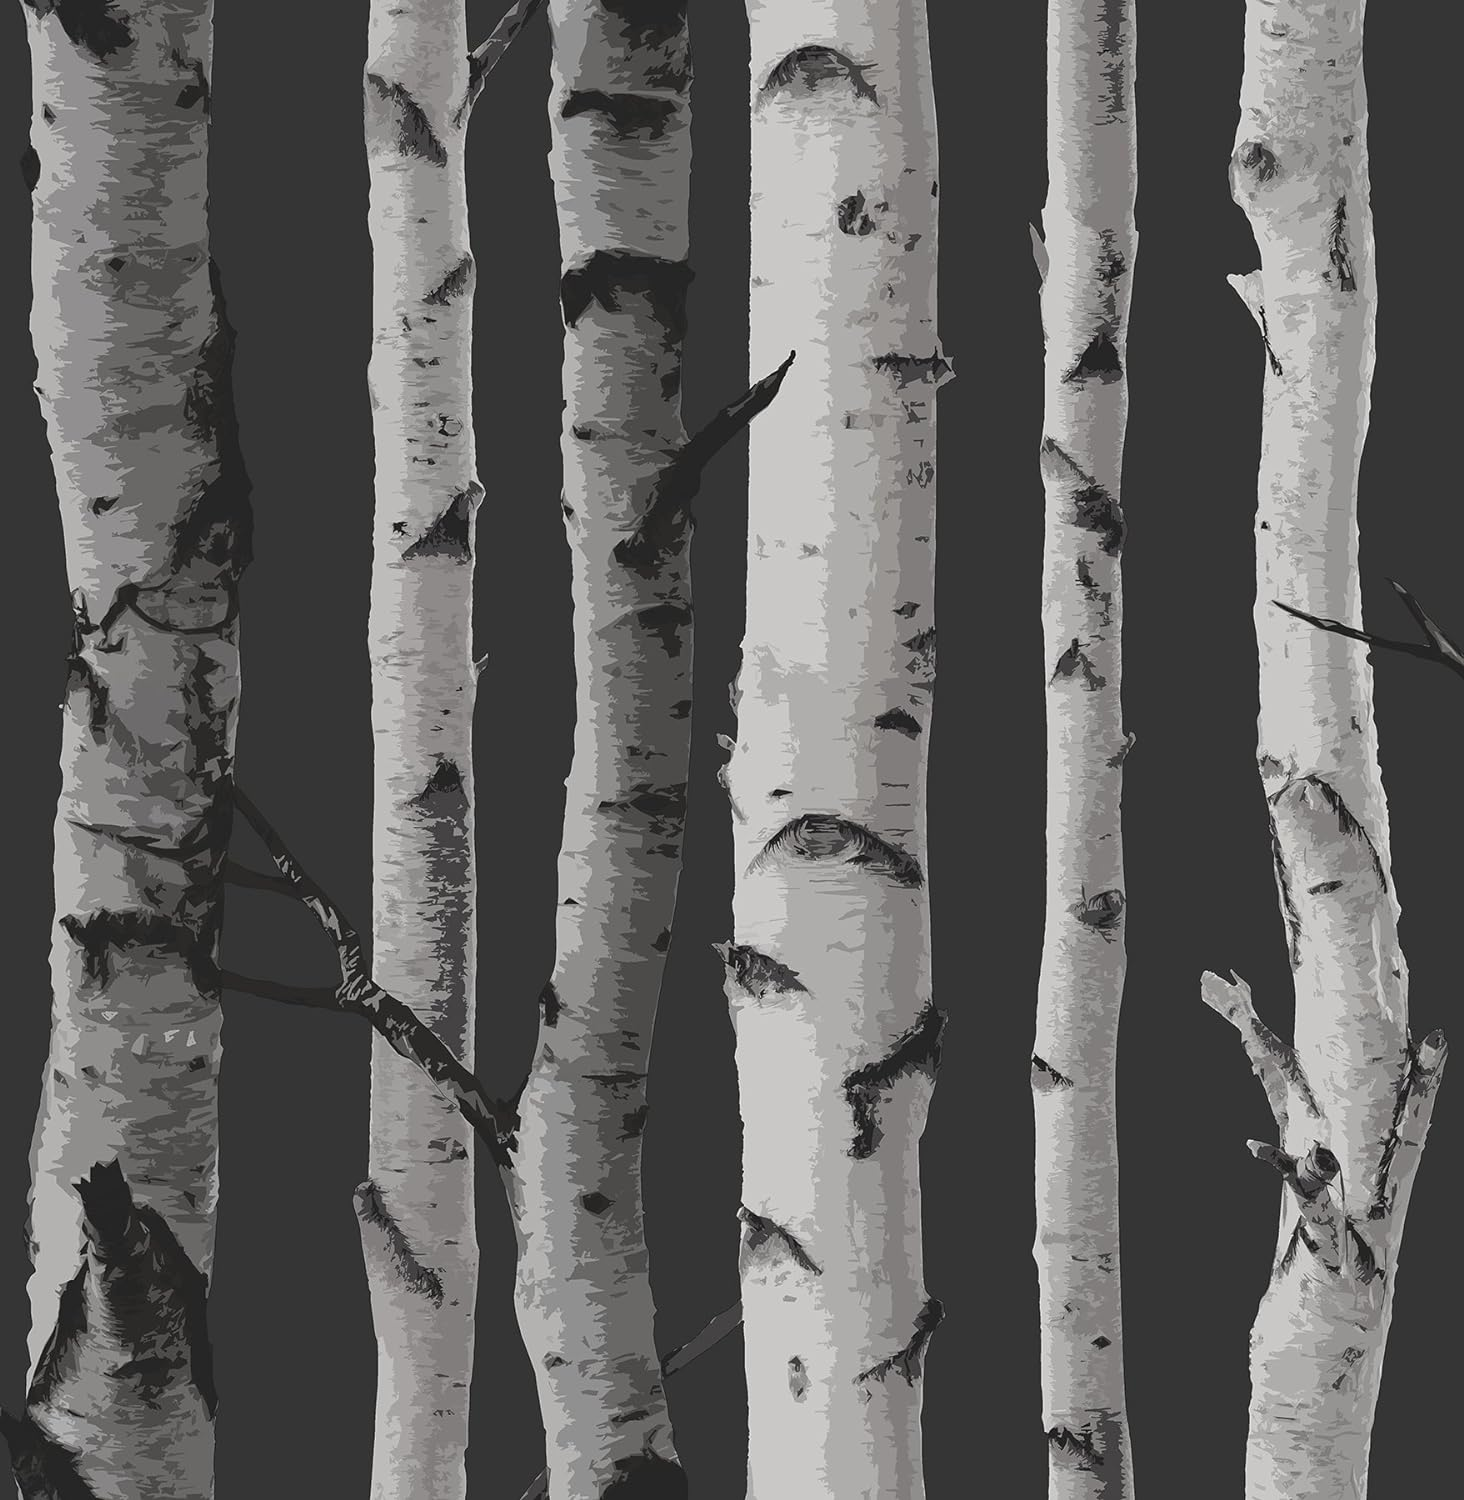
\includegraphics[width=0.5\linewidth]{birch.jpg}
\end{center}

The \lstinline|\includegraphics[<options>]{<file name>}| command is provided by the \texttt{graphicx} package which is internally loaded by the \texttt{tikz} package.

The \hyperref[sec:custom_settings.tex]{\texttt{custom\_settings.tex}} file includes the setting:
\begin{center}
    \lstinline|\graphicspath{{./Images/}}|
\end{center}
which establishes that \LaTeX\ should look for your image files in the \texttt{Images} folder by default.

For more information on including images in your document, see \href{https://en.wikibooks.org/wiki/LaTeX/Importing_Graphics}{here}.

%%%%%%%%%%%
% Resources
%%%%%%%%%%%
\section{Resources}
\label{sec:resources}

\subsection{Tools and Services}
\label{sec:tools_and_services}
\begin{itemize}
    \item \href{https://www.overleaf.com/}{Overleaf.com}
    \item \href{https://detexify.kirelabs.org/classify.html}{Detexify}
    \item \href{https://texnique.xyz/}{\TeX{}nique}
\end{itemize}

\subsection{Books and References}
\label{sec:books_and_references}
\begin{itemize}
    \item \href{https://www.overleaf.com/learn}{Overleaf Documentation}
    \item \href{https://tobi.oetiker.ch/lshort/lshort.pdf}{The Not So Short Introduction to \LaTeX}
    \item \href{https://www.latex-project.org/help/books/}{LaTeX-Project.org: \TeX\ and \LaTeX\ Books}
    \item \href{https://en.wikibooks.org/wiki/LaTeX}{The \LaTeX\ Wikibook}
    \item \href{https://tug.org/begin.html}{TUG.org: Starting out with \TeX, \LaTeX, and friends}
    \item \href{https://ctan.org/pkg/comprehensive}{The Comprehensive \LaTeX\ Symbol List}
    \item \href{https://www.ams.org/publications/authors/faq/author-faq}{American Mathematical Society \LaTeX\ FAQ}
    \item \href{https://castel.dev/}{castel.dev}
\end{itemize}

